\documentclass[12pt]{article}

\usepackage[a4paper,margin=1.7cm]{geometry}
\usepackage{graphicx}
\usepackage{booktabs}
\usepackage{array}
\usepackage{enumitem}
\usepackage{siunitx}
\usepackage{multicol}
\usepackage{caption}

\sisetup{
  per-mode=symbol,
  detect-all,
  round-mode=places,
  round-precision=2
}

\setlength{\parindent}{0pt}
\setlength{\parskip}{6pt}

\begin{document}

\begin{center}
{\LARGE Distance--Time Graphs Worksheet}\\
\vspace{2mm}
\end{center}

\vspace{2mm}

\textbf{Key idea:} Velocity is the \textbf{gradient} of a distance--time graph.
\[
m=\frac{\Delta y}{\Delta x}
\quad\text{(units: \si{m/s})}
\]

\vspace{2mm}
\hrule
\vspace{4mm}

% ===================== GRAPH 1 =====================
\section*{Graph 1}

\begin{center}
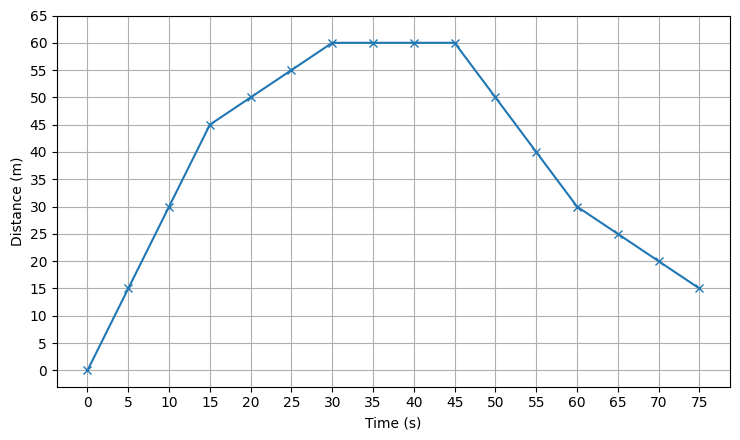
\includegraphics[width=\linewidth]{graph1.png}
\end{center}

\begin{enumerate}[label=\textbf{1.\arabic*}]
  \item Identify the time interval where the object is stationary. Give the interval in seconds.
  \vspace{1.2cm}

  \item Calculate the velocity between \textbf{0 and 15s} of the journey.
  (Tip: remember that in order to calculate the velocity you need to determine the gradient)
  \vspace{2.4cm}

  \item In which section of the graph is the object traveling the \textbf{fastest}? Explain how you can tell from the graph.
  \vspace{1.4cm}

  \item At what time does the object reach its \textbf{maximum distance}? What is that maximum distance?
  \vspace{1.4cm}

  \item Describe the motion of the object from start to finish (one or two sentences).
  \vspace{3cm}
\end{enumerate}

\vspace{3mm}
\hrule
\vspace{4mm}

% ===================== GRAPH 2 =====================
\section*{Graph 2}

\begin{center}
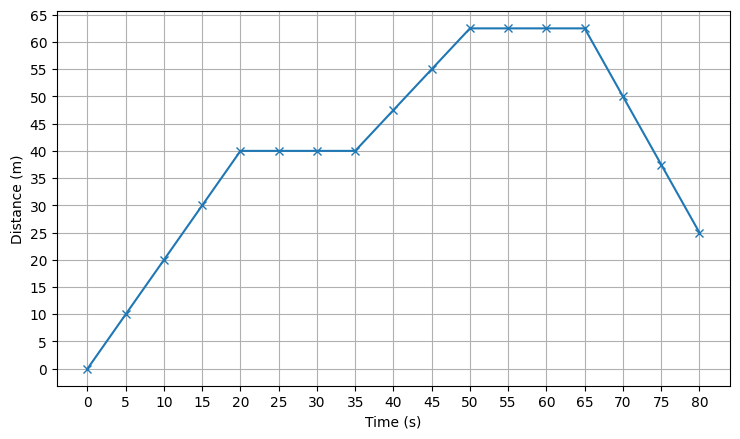
\includegraphics[width=\linewidth]{graph2.png}
\end{center}

\begin{enumerate}[label=\textbf{2.\arabic*}]
  \item Identify the time intervals where the object is stationary. Give both the intervals in seconds.
  \vspace{1.2cm}

  \item Calculate the velocity between \textbf{35 and 50s} of the journey.
  \vspace{2.4cm}

  \item Which section shows the object start travelling back towards the start? How can you tell?
  \vspace{1.2cm}

  \item Determine the object’s distance at $t=\SI{45}{s}$.
  \vspace{1.2cm}

  \item Which section is the \textbf{fastest?} Explain using the idea of gradient.
  \vspace{3cm}
\end{enumerate}

\vspace{3mm}
\hrule
\vspace{4mm}

% ===================== GRAPH 3 (students sketch) =====================
\section*{Graph 3}

\textbf{Instructions:} Use the blank grid below and plot the data points from the table. Join points with straight lines.

\begin{center}
\captionsetup{type=table}
\caption{Graph 3 data}
\vspace{-2mm}

\begin{tabular}{@{}l*{16}{c}@{}}
\toprule
Time (s) &
0 & 5 & 10 & 15 & 20 & 25 & 30 & 35 & 40 & 45 & 50 & 55 & 60 & 65 & 70 & 75 \\
Distance (m) &
0 & 20 & 40 & 42.5 & 45 & 47.5 & 47.5 & 47.5 & 47.5 & 40 & 32.5 & 25 & 20 & 15 & 10 & 5 \\
\bottomrule
\end{tabular}
\end{center}

\begin{center}
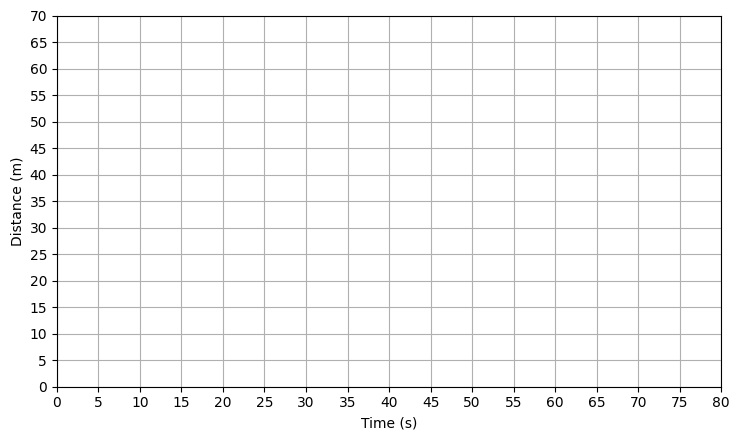
\includegraphics[width=\linewidth]{graphblank.png}
\end{center}

\begin{enumerate}[label=\textbf{3.\arabic*}]
  \item From your sketch, identify the stationary section (give the time interval).
  \vspace{1.2cm}

  \item Calculate the velocity between \textbf{0 and 10s} of the journey.
  \vspace{2.4cm}

  \item Which section is the \textbf{fastest}? Explain your reasoning.
  \vspace{1.6cm}

  \item At what time does the object first reach a distance of about \SI{40}{m}?
  \vspace{1.2cm}

  \item Describe the motion from start to finish (one or two sentences).
  \vspace{3cm}
\end{enumerate}

% ===================== GRAPH 4 (students sketch) =====================
\newpage
\section*{Graph 4 (You must sketch this graph)}

\textbf{Instructions:} Use the blank grid below and plot the data points from the table. Join points with straight lines.

\begin{center}
\captionsetup{type=table}
\caption{Graph 4 data}
\vspace{-2mm}

\begin{tabular}{@{}l*{17}{c}@{}}
\toprule
Time (s) &
0 & 5 & 10 & 15 & 20 & 25 & 30 & 35 & 40 & 45 & 50 & 55 & 60 & 65 & 70 & 75 & 80 \\
Distance (m) &
0 & 7.5 & 15 & 22.5 & 30 & 40 & 50 & 60 & 60 & 60 & 60 & 55 & 50 & 45 & 35 & 25 & 15 \\
\bottomrule
\end{tabular}
\end{center}

\begin{center}
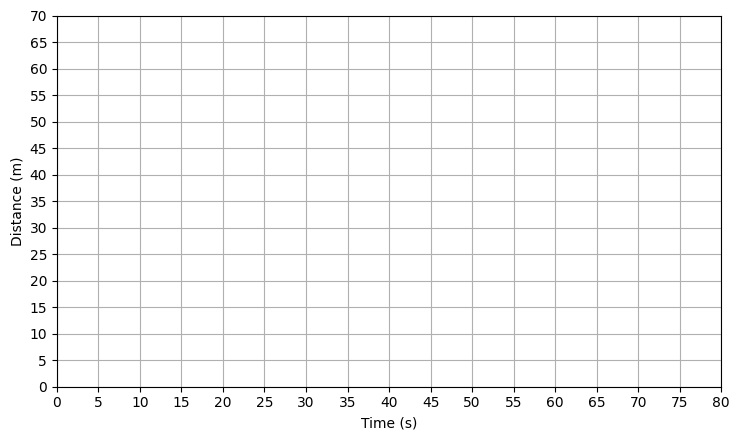
\includegraphics[width=\linewidth]{graphblank.png}
\end{center}

\begin{enumerate}[label=\textbf{4.\arabic*}]
  \item Identify any stationary interval from your sketch (give time interval).
  \vspace{1.2cm}

  \item Calculate the velocity \textbf{for each} straight-line section of the journey.
  \vspace{9.6cm}

  \item What is the average speed for the entire outbound section of the journey? 
  (Tip: in order to determine average speed, you can use the speed, distance, time formula using data from the graph)
  \vspace{4.8cm}

  \item Which section has the greatest negative gradient? (give the time interval). What does that mean physically?
  \vspace{2.4cm}

  \item Using the velocity you determined earlier, calculate the exact distance at $t=\SI{12}{s}$.
  \vspace{1.4cm}
\end{enumerate}

\newpage
\section*{Mark Scheme}

% ===================== GRAPH 1 =====================
\subsection*{Graph 1}

\begin{enumerate}[label=\textbf{1.\arabic*}]
  \item Stationary from \textbf{30--45 s}.

  \item Velocity from 0--15 s:  
  $v = 3.0\,\si{m/s}$

  \item Fastest section: \textbf{0--15 s}  
  (Steepest gradient.)

  \item Maximum distance: \textbf{60 m} at \textbf{30--45 s}.

  \item Description:  
  The object moves away quickly, slows down, stops, then returns towards the start.
\end{enumerate}

\hrule
\vspace{4mm}

% ===================== GRAPH 2 =====================
\subsection*{Graph 2}

\begin{enumerate}[label=\textbf{2.\arabic*}]
  \item Stationary from \textbf{20--35 s} and \textbf{50--65 s}.

  \item Velocity from 35--50 s:  
  $v = 1.5\,\si{m/s}$

  \item Returns towards the start from \textbf{65--80 s}  
  (Negative gradient.)

  \item Distance at 45 s: \textbf{55 m}.

  \item Fastest section: \textbf{65--80 s}  
  (Largest gradient magnitude.)
\end{enumerate}

\hrule
\vspace{4mm}

% ===================== GRAPH 3 =====================
\subsection*{Graph 3}

\begin{enumerate}[label=\textbf{3.\arabic*}]
  \item Stationary from \textbf{30--40 s}.

  \item Velocity from 0--10 s:  
  $v = 4.0\,\si{m/s}$

  \item Fastest section: \textbf{0--10 s}  
  (Steepest gradient.)

  \item Reaches 40 m at \textbf{10 s}.

  \item Description:  
  The object moves away very quickly, slows down, stops, then returns towards the start.
\end{enumerate}

\hrule
\vspace{4mm}

% ===================== GRAPH 4 =====================
\subsection*{Graph 4}

\begin{enumerate}[label=\textbf{4.\arabic*}]
  \item Stationary from \textbf{35--50 s}.

  \item Velocities:
  \begin{itemize}
    \item 0--20 s: $1.5\,\si{m/s}$
    \item 20--35 s: $2.0\,\si{m/s}$
    \item 35--50 s: $0\,\si{m/s}$
    \item 50--65 s: $-1.0\,\si{m/s}$
    \item 65--80 s: $-2.0\,\si{m/s}$
  \end{itemize}

  \item Average speed (outbound 0--35 s):  
  $\approx 1.7\,\si{m/s}$

  \item Greatest negative gradient: \textbf{65--80 s}  
  Meaning: object is returning towards the start fastest.

  \item Distance at 12 s:  
  $d = v \times t = 1.5 \times 12 = \textbf{18 m}$
\end{enumerate}


\end{document}
